\chapter{2 Zones house model 7R4C network}

The 4R-7C house model structure is implemented as described below:
	
\begin{figure}[H]
	\centering
	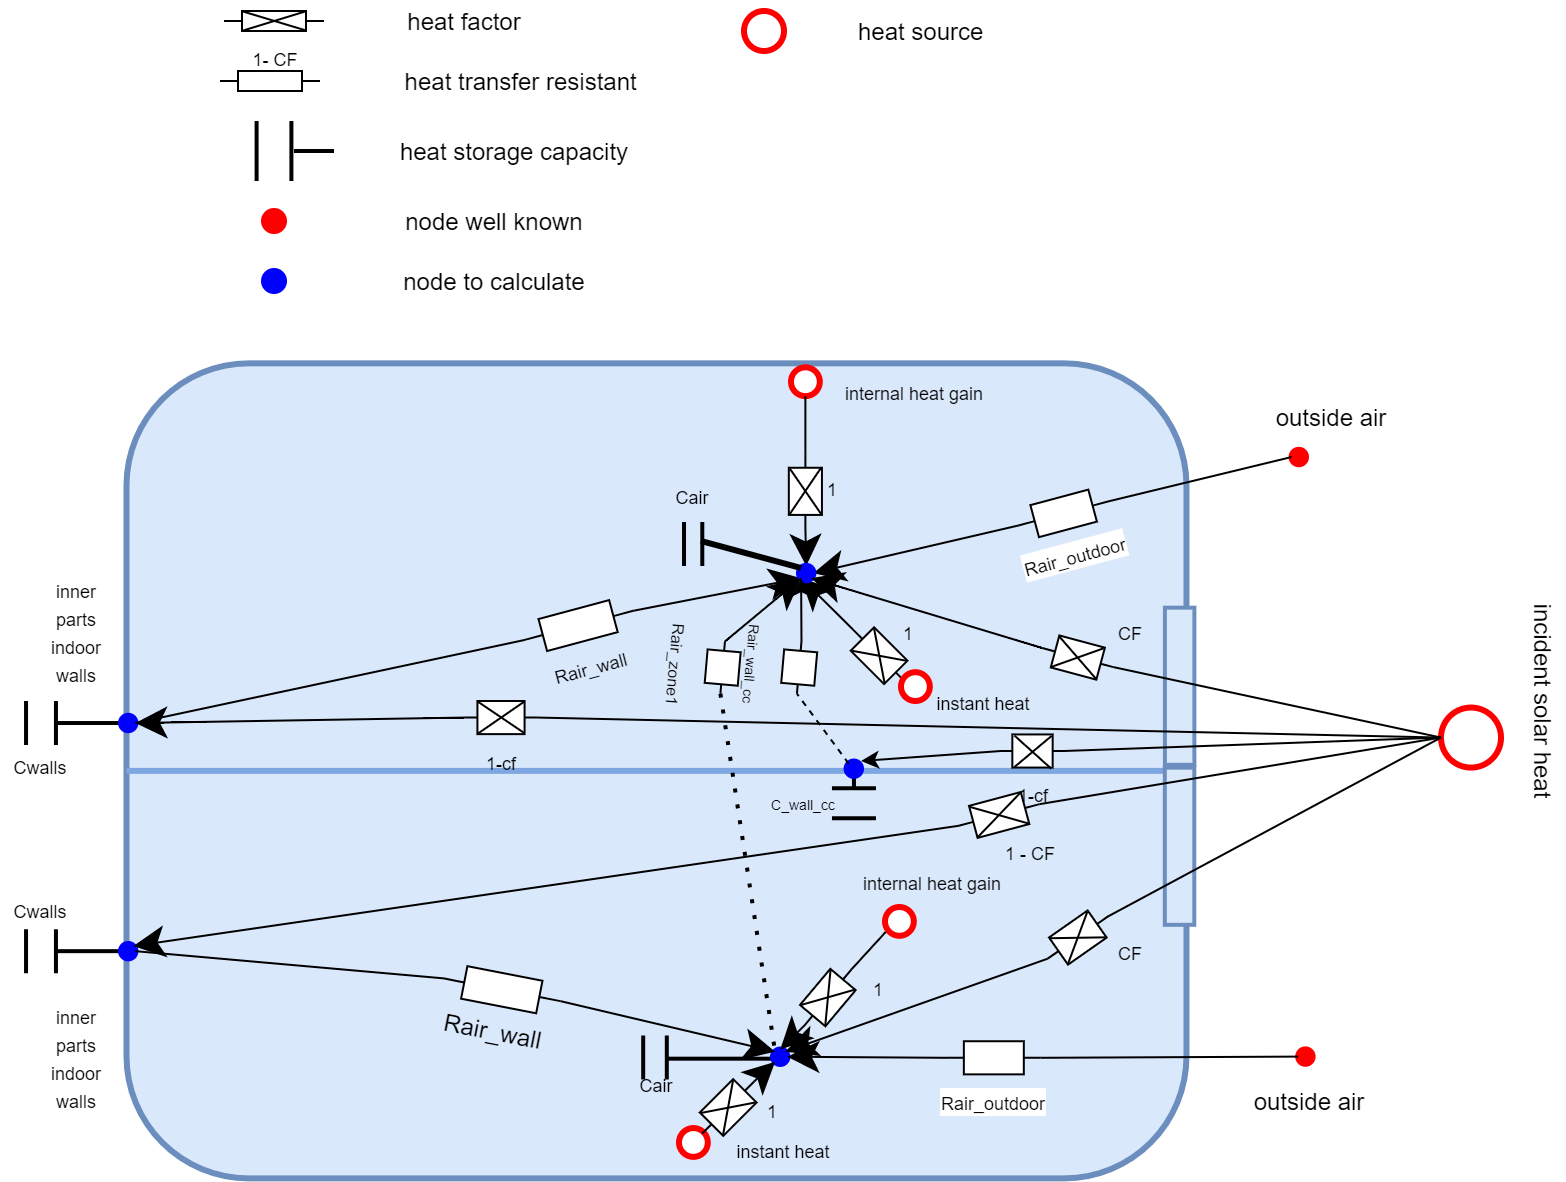
\includegraphics[width=1.0\columnwidth]{Pictures/House_electrical_circuits overview.png}
	\caption[Short title]{Schematic of a 2 zones house model}
	\label{fig:schema7R4C}
	\end{figure} 
	
The equivalent electrical 7R-4C network with components and topology is given in Fig. \ref{fig:elec7R4C}.

\begin{figure}[H]
	\centering
	
\includegraphics[width=1.0\columnwidth]{Pictures/2_Zones_house_circuits.png}
	\caption[Short title]{R-C circuits of 2 zones house model}
	\label{fig:elec7R4C}
	\end{figure}

with:\\
\begin{itemize}
    \item \texttt{T\_outdoor} : outdoor temperature [$\degr C$] 
    \item \texttt{T\_air\_1}  : zone 1 air temperature [$\degr C$]
    \item \texttt{T\_walls}   : wall temperature [$\degr C$]
    \item \texttt{T\_air\_2}  : zone 2 air temperature [$\degr C$]
    \item \texttt{T\_cc}      : temperature of the concrete layer between zone 1 and zone 2 [$\degr C$]
    \item \texttt{R\_air\_1\_outdoor} : outdoor resistance valus.
    \item \texttt{R\_wall\_1} : walls resistance value.
    \item \texttt{R\_wall\_2} : walls resistance value.
    \item \texttt{R\_cc}      : concrete resistance value.
    \item \texttt{R\_air\_12} : resistance value of air flow from zone 1 to zone 2.
    \item \texttt{R\_air\_21} : resistance value of air flow from zone 2 to zone 1.

\end{itemize}
\newpage